\documentclass{VUMIFInfKursinis}
\usepackage{algorithmicx}
\usepackage{algorithm}
\usepackage{algpseudocode}
\usepackage{amsfonts}
\usepackage{amsmath}
\usepackage{bm}
\usepackage{color}
\usepackage{graphicx}
% \usepackage{hyperref}  % Nuorodų aktyvavimas
\usepackage{url}


% Titulinio aprašas
\university{Vilniaus universitetas}
\faculty{Matematikos ir informatikos fakultetas}
\institute{Informatikos institutas}  % Užkomentavus šią eilutę - institutas neįtraukiamas į titulinį
\department{Informatikos katedra}
\papertype{Operacinių sistemų pirmoji užduotis}
\title{Multiprograminės OS projektas}
%\titleineng{Modeling of Risk Management Process}
\status{3 kurso 1 grupės studentas}
\author{Dominykas Marma}
% \secondauthor{Vardonis Pavardonis}   % Pridėti antrą autorių
\supervisor{Mantas Grubliauskis}
\date{Vilnius \\ \the\year}

% Nustatymai
% \setmainfont{Palemonas}   % Pakeisti teksto šriftą į Palemonas (turi būti įdiegtas sistemoje)
\bibliography{bibliografija} 

\begin{document}
\maketitle

\tableofcontents

\section{Procesai}

Procesai - vykdomosios programos su esamomis registrų reikšmėmis ir savo kintamaisiais.

\subsection{Procesų būsenos}

\begin{itemize}
	\item Vykdomas - turi procesorių.
	\item Pasiruošęs - vienintelis trūkstamas resursas yra procesorius.
	\item Blokuotas - prašo resurso (išskyrus procesorių).
	\item Pasiruošęs sustabdytas
	\item Blokuotas sustabdytas
\end{itemize}

\subsection{Procesų būsenų kitimas}

\begin{figure}[H]
	\centering	
	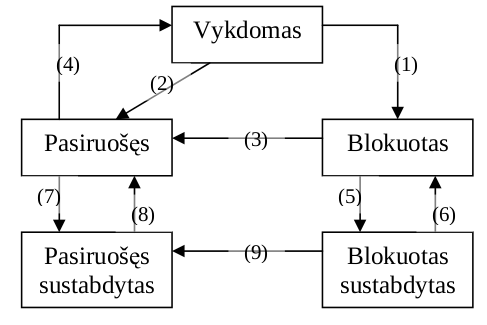
\includegraphics[scale=0.6]{img/busenu-kitimas}
	\caption{Proceso būsenų kitimo diagrama}   % Antraštė įterpiama po paveikslėlio
	\label{img:busenu-kitimas}
\end{figure}

\begin{enumerate}
	\item Vykdomas procesas blokuojasi jam prašant ir negavus resurso.
	\item Vykdomas procesas tampa pasiruošusiu atėmus iš jo procesorių dėl kokios
	nors priežasties (išskyrus resurso negavimą).
	\item Blokuotas procesas tampa pasiruošusiu, kai yra suteikiamas reikalingas
	resursas.
	\item Pasiruošę procesai varžosi dėl procesoriaus. Gavęs procesorių procesas tampa
	vykdomu.
	\item Procesas gali tapti sustabdytu blokuotu, jei einamasis procesas jį sustabdo, kai
	jis jau ir taip yra blokuotas.
	\item Procesas tampa blokuotu iš blokuoto sustabdyto, jei einamasis procesas nuima
	būseną sustabdytas.
	\item Procesas gali tapti pasiruošusiu sustabdytu, jei einamasis procesas jį sustabdo,
	kai jis yra pasiruošęs.
	\item Procesas tampa pasiruošusiu iš pasiruošusio sustabdyto, jei einamasis procesas
	nuima būseną sustabdytas
	\item Procesas tampa pasiruošusiu sustabdytu iš blokuoto sustabdyto, jei procesui
	yra suteikiamas jam reikalingas resursas.
\end{enumerate}


\subsection{Planuotojas}

Planuotojo paskirtis - atimti procesorių iš procceso, peržvelgti pasiruošųsių procesų sąrašą ir tinkamiausiam iš jų perduoti procesorių.

\begin{figure}[H]
	\centering	
	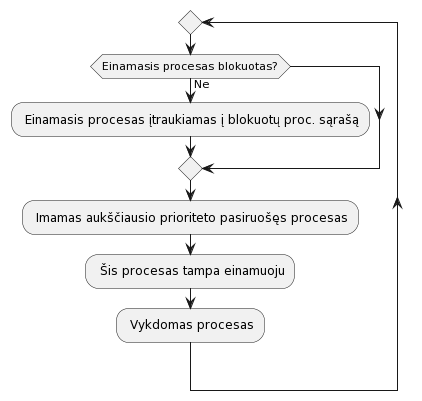
\includegraphics[scale=0.65]{img/scheduler}
	\caption{Planuotojo diagrama}   % Antraštė įterpiama po paveikslėlio
	\label{img:scheduler}
\end{figure}

\subsubsection{Prioritetai}

Visi procesai turi prioritetus nuo 0 iki 20, kuo didesnis prioritetas, tuo didesnė tikimybė, kad procesas bus vykdomas.

\subsection{Resursų paskirstytojas}

Resursų paskirstytojo paskirtis - suteikti paprašytą resurso elementų kiekį procesui.

\subsection{Procesų primityvai}

\begin{itemize}
	\item Kurti procesą - perduodama nuoroda į tėvinį procesą ir kūrimo parametrai.
	\item Naikinti procesą - perduodama naikinama proceso nuoroda. Taip yra sunaikinami visi šio proceso vaikiniai procesai.
	\item Stabdyti procesą - perduodama stabdomo proceso nuoroda.
\end{itemize}

\subsection{Procesų kūrimo ir trynimo lentelė}

\begin{table}[H]\footnotesize
	\centering
	\caption{Procesų kūrimo ir trynimo lentelė}    % Antraštė įterpiama prieš lentelę
	\begin{tabular}{|c|c|c|}
		\hline
		Proceso pavadinimas & Procesas, kuris jį sukuria & Procesas, kuris jį ištrina \\
		\hline
		StartStop & Niekas (sistemos pradžioje pasileidžia) & Niekas (pats išsijungia) \\
		\hline
		ReadFromInterface & StartStop & StartStop\\
		\hline
		JCL & StartStop & StartStop \\
		\hline
		MainProc & StartStop & StartStop \\
		\hline
		JobGovernor & MainProc & MainProc \\
		\hline
		VirtualMachine & JobGovernor & JobGovernor \\
		\hline
		Interrupt & StartStop & StartStop \\
		\hline
		PrintLine & StartStop & StartStop \\
		\hline
		FileSystem & StartStop & StartStop \\
		\hline
		Idle & StartStop & StartStop \\
		\hline
	\end{tabular}
	\label{tab:duomenys}
\end{table}

\subsection{StartStop}

Paskirtis - darbo pradžioje sukurti resursus ir sisteminius procesus.

\begin{figure}[H]
	\centering	
	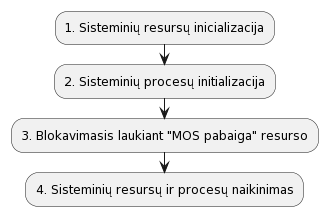
\includegraphics[scale=0.65]{img/StartStop}
	\caption{Proceso StartStop diagrama}   % Antraštė įterpiama po paveikslėlio
	\label{img:StartStop}
\end{figure}

\subsection{ReadFromInterface}

Paskirtis - gavus informaciją iš įvedimo srauto atlikti pirminį jos apdorojimą, atiduoti informaciją procesui JCL, tolesniam apdorojimui.

\begin{figure}[H]
	\centering	
	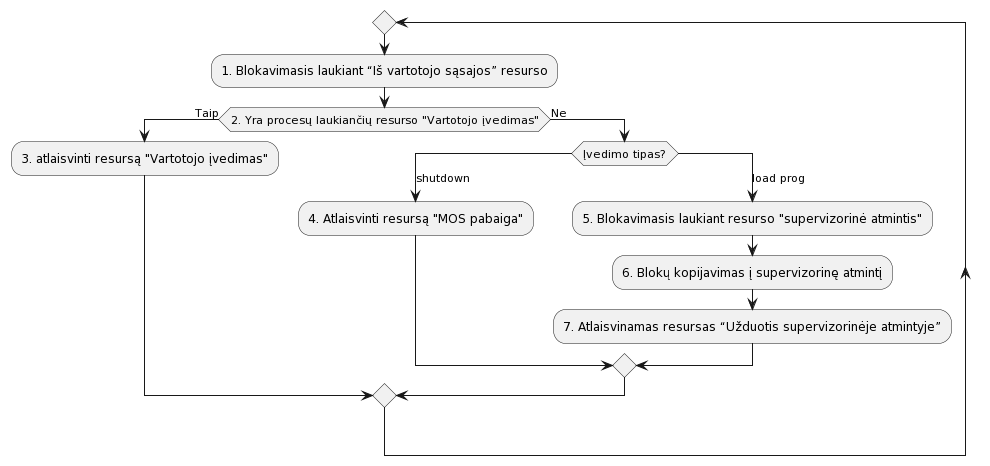
\includegraphics[scale=0.30]{img/ReadFromInterface}
	\caption{Proceso ReadFromInterface diagrama}   % Antraštė įterpiama po paveikslėlio
	\label{img:ReadFromInterface}
\end{figure}

\subsection{JCL}

JCL paskirtis - patikrinti perkeltos programos korektiškumą.

\begin{figure}[H]
	\centering	
	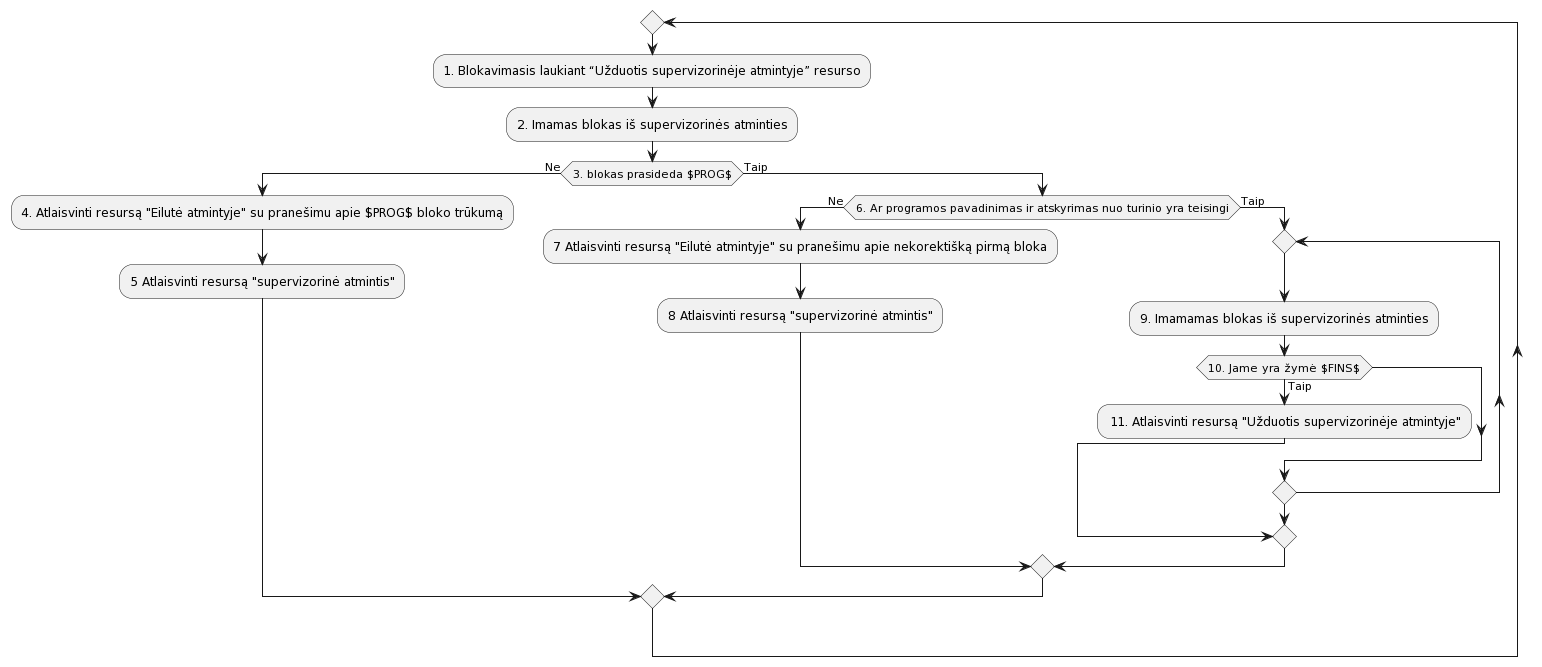
\includegraphics[scale=1.5]{img/JCL}
	\caption{Proceso JCL diagrama}   % Antraštė įterpiama po paveikslėlio
	\label{img:JCL}
\end{figure}

\subsection{MainProc}

MainProc paskirtis - kurti ir naikinti procesus JobGovernor.

\begin{figure}[H]
	\centering	
	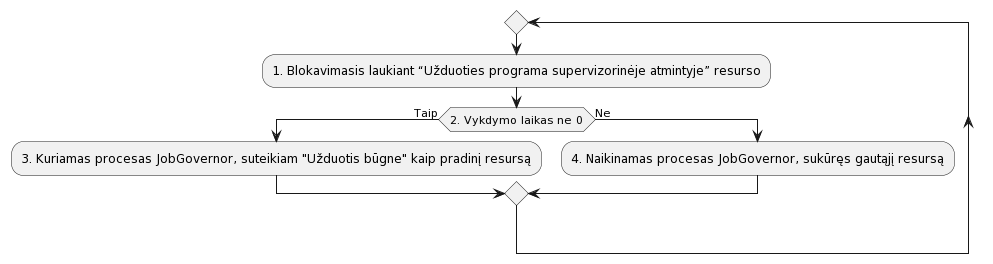
\includegraphics[scale=0.40]{img/MainProc}
	\caption{Proceso MainProc diagrama}   % Antraštė įterpiama po paveikslėlio
	\label{img:MainProc}
\end{figure}

\subsection{JobGovernor}

JobGovernor paskirtis - kurti, naikinti VIrtualMachine ir padėti tvarkyti pertraukimus.

\begin{figure}[H]
	\centering	
	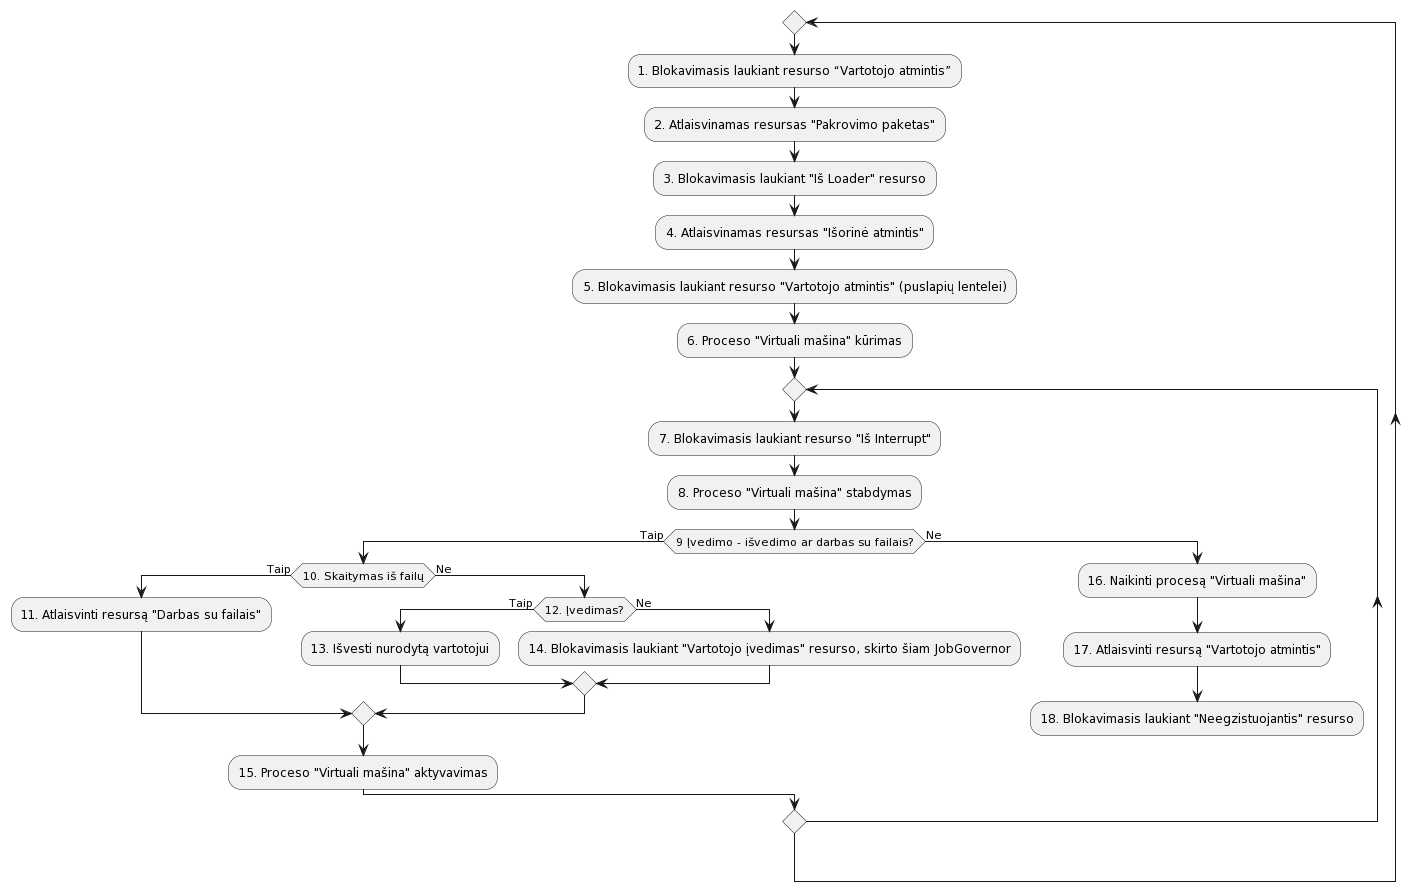
\includegraphics[scale=0.3]{img/JobGovernor}
	\caption{Proceso JobGovernor diagrama}   % Antraštė įterpiama po paveikslėlio
	\label{img:JobGovernor}
\end{figure}

\subsection{VirtualMachine}

VirtualMachine paskirtis - vykdyti vartotojo užduoties programą.

\begin{figure}[H]
	\centering	
	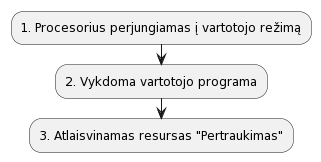
\includegraphics[scale=0.65]{img/VirtualMachine}
	\caption{Proceso VirtualMachine diagrama}   % Antraštė įterpiama po paveikslėlio
	\label{img:VirtualMachine}
\end{figure}

\subsection{Interrupt}

Proceso Interrupt paskirtis - reaguoti į pertraukimus, kilusius virtualios mašinos darbo metu.

\begin{figure}[H]
	\centering	
	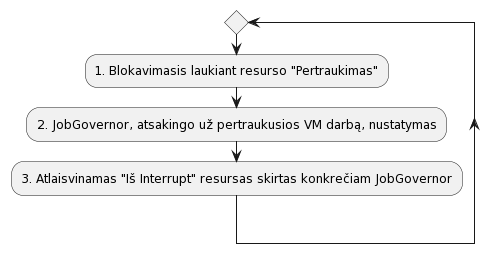
\includegraphics[scale=0.65]{img/Interrupt}
	\caption{Proceso Interrupt diagrama}   % Antraštė įterpiama po paveikslėlio
	\label{img:Interrupt}
\end{figure}

\subsection{PrintLine}

Proceso PrintLine paskirtis - į išvedimo srautą pasiųsti pranešimą.

\begin{figure}[H]
	\centering	
	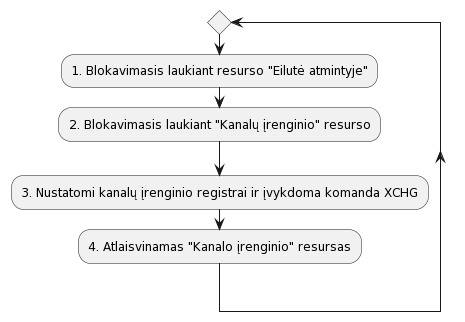
\includegraphics[scale=0.65]{img/PrintLine}
	\caption{Proceso PrintLine diagrama}   % Antraštė įterpiama po paveikslėlio
	\label{img:PrintLine}
\end{figure}

\subsection{FileSystem}

Proceso paskirtis - aptarnauti veiksmus, susijusius su failų sistema.

\begin{figure}[H]
	\centering	
	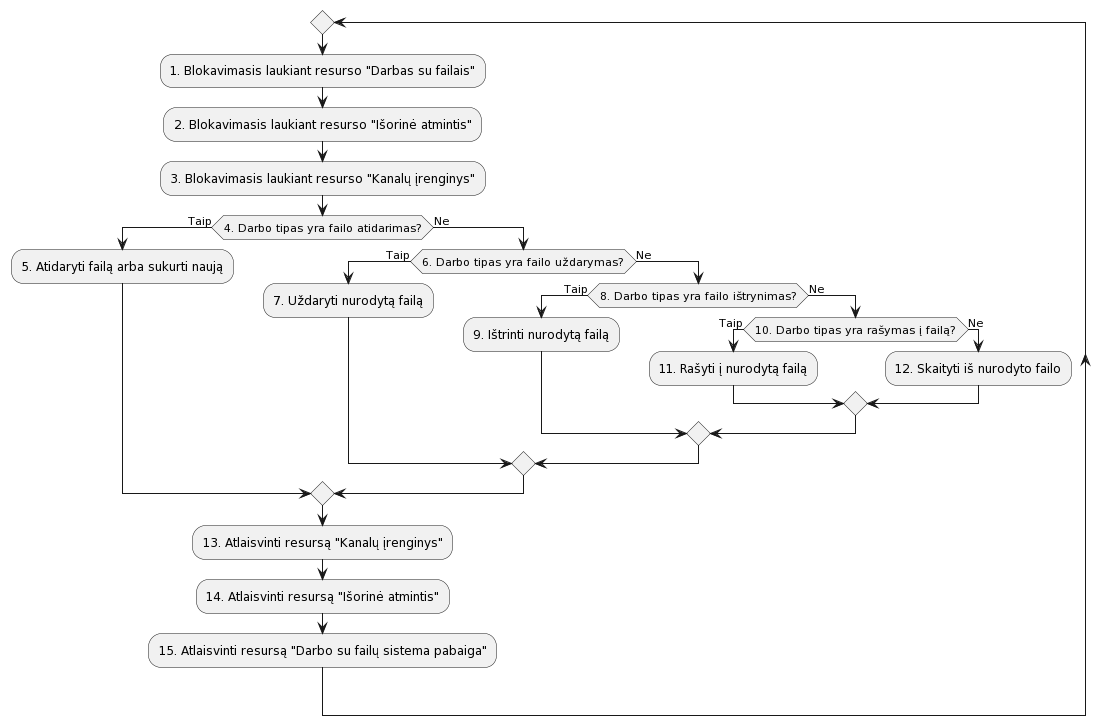
\includegraphics[scale=0.35]{img/FileSystem}
	\caption{Proceso FileSystem diagrama}   % Antraštė įterpiama po paveikslėlio
	\label{img:FileSystem}
\end{figure}

\subsection{Idle}

Proceso Idle paskirtis - būti vykdomam, kai nėra kitų pasiruošusių procesų. Šis procesas visada turi žemiausią įmanomą prioritetą.

\begin{figure}[H]
	\centering	
	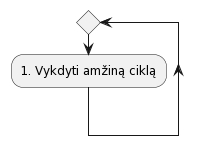
\includegraphics[scale=0.65]{img/Idle}
	\caption{Proceso Idle diagrama}   % Antraštė įterpiama po paveikslėlio
	\label{img:Idle}
\end{figure}


\section{Resursai}

Resursai yra tai, dėl ko varžosi procesai. Dėl resursų trūkumo procesai blokuojasi, gavę reikiamą resursą, procesai tampa pasiruošusiais.

\subsection{Resursų lentelė}

% https://tex.stackexchange.com/questions/40561/table-with-multiple-lines-in-some-cells
% p prie parametrų turbūt, kad būtų multiline
\begin{table}[H]\footnotesize
	\centering
	\caption{Resursų lentelė}    % Antraštė įterpiama prieš lentelę
	\begin{tabular}{|c|c|c|c|}
		\hline
		Resurso pavadinimas & Resursą kuria & Resursą atlaisvina & Dėl resurso blokuojasi \\
		\hline
		\multicolumn{4}{c}{Sisteminiai}\\
		\hline
		Kanalų įrenginys & StartStop & \begin{tabular}{@{}c@{}}PrintLine, JobGovernor,\\ FileSystem \end{tabular} & \begin{tabular}{@{}c@{}}PrintLine, JobGovernor,\\ FileSystem \end{tabular}\\
		\hline
		Supervizorinė atmintis & StartStop & JobGovernor, JCL & ReadFromInterface \\
		\hline
		Vartotojo atmintis & StartStop & JobGovernor & JobGovernor\\
		\hline
		Išorinė atmintis & StartStop & FileSystem & FileSystem \\
		\hline
		\multicolumn{4}{c}{Programiniai}\\
		\hline
		MOS pabaiga & StartStop & ReadFromInterface & StartStop \\
		\hline
		Iš vartotojo sąsajos & StartStop & & ReadFromInterface \\
		\hline
		Užduotis supervizorinėje atmintyje & StartStop & ReadFromInterface & JCL \\
		\hline
		Užduoties programa supervizorinėje atmintyje & StartStop & JCL & MainProc \\
		\hline
		Eilutė atmintyje & StartStop &     \begin{tabular}{@{}c@{}}ReadFromInterface, JCL,\\ JobGovernor \end{tabular} & PrintLine\\
		\hline
		Iš Interrupt & StartStop & Interrupt & JobGovernor\\
		\hline
		Vartotojo įvedimas & StartStop & ReadFromInterface & JobGovernor \\
		\hline 
		Vartotojo įvedimas gautas & StartStop & JobGovernor & ReadFromInterface \\
		\hline 
		Pertraukimas & StartStop & VirtualMachine & Interrupt\\
		\hline 
		Darbas su failais & StartStop & JobGovernor & FileSystem \\
		\hline
		Darbo su failais pabaiga & StartStop & FileSystem & JobGovernor \\
		\hline 
		Neegzistuojantis & StartStop & ------- & JobGovernor \\
		\hline
	\end{tabular}
	\label{tab:resursu_lentele}
\end{table}

\section{Procesų klasių aprašai}

\subsection{Kernelio aprašas}

TKernel - klasė realizuojanti OS branduolį. Čia laikomi procesų, resursų sąrašai, planuotojas bei kitos reikalingos klasės.

TKernel susideda iš šių dalių:

\begin{itemize}
	\item FProcesses: TProcessList (bendras visų, esančių sistemoje, procesų sąrašas)
	\item FResources: TresourceList (bendras visų, sistemoje esančių, resursų sąrašas)
	\item FReadyProc: TProcessList (pasiruošusių procesų sąrašas)
	\item ActiveProcess: TProcess (dabar veikiantis procesas)
	\item FRealMachine: TRealMachine (nuoroda į realią mašiną)
\end{itemize} 

\subsection{Proceso klasės aprašas}

Proceso klasė TProcess susideda iš šių dalių:

\begin{itemize}
	\item FID: Integer (unikalus objekto id)
	\item FSavedRegisters: TSavedReisters (išsaugota registrų būsena)
	\item FCreatedRes: TResourceList (sukurtų resursų sąrašas)
	\item FState: TProcessState (kuriame žingsnyje yra procesas)
	\item FPriority: Integer
	\item FParent: TProcess (tėvinio proceso nuoroda)
	\item FChildren: TProcessList
\end{itemize}

\subsection{Resurso klasės aprašas}

Resurso klasė TResource susideda iš šių dalių:

\begin{itemize}
	\item FID: Integer (unikalus objekto id)
	\item FList: TElementList (nuoroda į resurso elementų sąrašą)
	\item FWaitingProcesses : TProcessList (nuoroda į šio resurso laukiančių procesų sąrašą)
	\item FWaitingCount: TIntegerList (nuoroda į šio resurso laukiančių procesų paprašytų
	resurso kiekių sąrašą).
	\item FResourceList: TResourceList (nuoroda į visų resursų sąrašą)
\end{itemize}

\subsection{Pagalbinės klasės}

Registrų būsena TSavedRegisters susidaro iš šių dalių:

\begin{itemize}
	\item R1: TWord
	\item R2: TWord
	\item R3: TWord
	\item CS: TDByte
	\item DS: TDByte
	\item IC: TDByte
	\item PI: TPIReg
	\item SI: TSIReg
	\item PTR: TDByte
	\item Mode: TByte
\end{itemize}

TPIReg ir TSIReg - aprašo ar dabar yra išauktas atitinkamas pertraukimas ir jei taip - koks jo tipas.

Resurso elemento klasė TResElement susideda iš šių dalių:

\begin{itemize}
	\item FElementList: TElementList (nuoroda į resurso elementų sąrašą, kuriame yra šis resurso elementas)
	\item FReceiver: TProcess (procesas, kuris turi gauti šį resurso elementą. Jei šio lauko
reikšmė lygi nil, tai laikoma, kad šį elementą gali gauti bet kuris procesas)
	\item FSender: TProcess (procesas, atlaisvinęs šį resurso elementą)
\end{itemize}

\printbibliography[heading=bibintoc] % Literatūros šaltiniai aprašomi
\appendix  % Priedai

\end{document}
